\section{Background and Definitions}\label{sec-background}
\reminder{I know we have discussed to put SampleClean before MVs. But I put SampleClean after MVs because it reads more natural.}
\subsection{Materialized View}\label{subsec-inc}




\subsubsection{Notation} \reminder{I put this section back to Sec 2 because Sec 2.1.2 uses undefined notations}

Given a database $\mathcal{D}$ which is a collection of relations $\{R_i\}$, a materialized view $S$ is the result of applying the relational expression $S_{def}$ to the database.
We use a multiset algebriac model (a set of elements with corresponding multiplicities) to represent the relations in the database $\mathcal{D}$ and the materialized view $S$.
We denote the multiset of insertions to a relation $R_i$ as $\Delta R_i$ and deletions as $\nabla R_i$.
In this paper, we refer to $\Delta R_i$ and $\nabla R_i$ as ``delta relations".
An update to a relation can be modeled as a deletion and then an insertion.
%In this work, we ignore \textbf{null} types and assume that each tuple in the relation has non-null attribute values.

We look at relation expressions for the view $S_{def}$ composed of the following operators:
\begin{itemize}\vspace{-.45em}
\item $\sigma_{\phi}(R)$: Selection select all tuples $r$ from $R$ that satisfy the restriction $\phi (r)$ \vspace{-.45em}
\item $\Pi_{a_1,a_2,...,a_k}(R)$: Projection select attributes $\{a_1,a_2,...,a_k\}$ from R \vspace{-.45em}
\item $\bowtie_{\phi (r1,r2)}(R_1,R_2)$: Join select all tuples in $R_1 \times R_2$ that satisfy $\phi (r_1,r_2)$.
\item $\gamma_{e}(R)$: Aggregation of R grouped by the relational expression $e(R)$.\footnote{A special case of this operator is $\delta$ the deduplication operator.}\vspace{-.45em}
\item $R_1 \dot{\cup} R_2$: Multiset union take a union of the two sets incrementing multiplicities.
\item $R_1 \dot{\cap} R_2$: Multiset intersection take an intersection of the set counting multiplicities.
\item $R_1 \dot{-} R_2$: Multiset set difference.
\end{itemize}


\subsubsection{View Maintenance}
\reminder{I would suggest you first talk about recomputation that is used to motivate incremental view maintenance, and then talk about how incremental view maintenance works, and finally say incremental view maintenance may not work for all views, thus recomputation is still necessary in some situations. In the end, you define maintenance }

Incremental maintenance of materialized views in multiset algebras has been well studied; see \cite{chirkova2011materialized} for a survey of the approaches. 
At a high-level, incremental maintenance algorithms typically consist of the following steps: for each leaf (relation) of the query tree of $S_{def}$ propagate $\Delta$ and $\nabla$ up the tree using composibility rules of delta relations, derive a \emph{change propagation formula} for $S$ in terms of deltas of subexpressions, and join this formula with the view to apply the changes. 
These rules are described in detail in \cite{DBLP:journals/vldb/KochAKNNLS14, DBLP:conf/pods/Koch10}.

However, even for the set of operators defined in the earlier section, there are some views for which full incremental maintenance is not possible and subexpressions have to recomputed. Consider the relation R(employeeid,country,salary) and view $S$ that calculates the \maxfunc salary of employees grouped by country. Under only insertions $\Delta R$, it is clear that the view can be maintained incrementally. 
However, if we allow deletions $\nabla R$ then it is unclear how to update a view if an employee with a maximal salary is deleted since we do not know the salary of the next highest employee. 

In cases like this, some recomputation is \underline{inevitable}. \reminder{ There's paper on this issue ``Incremental main- tenance for non-distributive aggregate functions," Try to avoid strong arguments. For example, you can say in this situation, it may be better to ... }
However, it turns out that SVC is general enough to handle both views that can be fully incrementally maintained and views that require partial or full recomputation.
In short, we say there is a \emph{maintenance strategy} $\mathcal{M}$ which is a relational expression that is a function of the database $\mathcal{D}$ and all the delta relations $\{\Delta R_i\} \cup \{\nabla R_i\}$ that updates the view.
%SVC takes the query tree of $\mathcal{M}$ as input and outputs a sampling plan and a query correction plan (Section ??). 
\reminder{Formally define the maintenance strategy here. Not }

\subsubsection{Why Materialized Views Go Stale}
The algebraic analysis of incremental maintenance informs us which views can be incrementally maintained.
However, there are many practical considerations of excuting these operations in real database systems and it may not always be feasible to immediately apply updates.
For example, in distributed systems record-at-a-time maintenance may be excessively affected by overheads and batching updates together can allows for amortization.
In other systems, such as Apache Spark, the immutability of data structures means that updates can sometimes incur overheads on the order of magnitude of recomputation (see experiments ??).
Finally, immediate scheduling of maintenance can place a bottleneck on updates to the base table which may result in degraded performance or worse having to drop updates to cope with load.

The main problem is that while immediate incremental maintenance has many advantages, the particulars of the database system and available resources often dictate how updates are propagated.
To address these challenges, deferred maintenance is an alternative solution.
The main insight of deferral is to avoid maintaining the view immediately and to schedule an update at a more convenient time either in a pre-set way or adaptively.
In deferred maintenance approaches, the user often accepts some degree of staleness for additional flexibility in scheduling.
For example, views can be updated at night when the system can use more resources to process the updates without affecting a critical application.
However, this also means that during the day the materialized view becomes increasingly stale as it was computed the night before.

These costs can also be deferred to query execution time.
In particular, we highlight a technique called lazy maintenance which applies updates to the view only when a user's query requires a row \cite{zhou2007lazy}.
While always fresh, both lazy maintenance and immediate maintenance hit a bottleneck when there are rapid updates, and this results increasingly degraded performance if a user wants to query a view.
The alternative is potentially unbounded staleness between maintenance cycles with deferred maintenance.
SVC addresses this problem from a new perspective, namely, can we accept some degree of bounded inaccuracy for increased performance.


\subsection{SampleClean: Fast and Accurate Query Processing on Dirty Data}

\reminder{Give the queries that SampleClean can support in this section. This makes the argument of Section 3.2.2 become easy. }

In our prior work on the SampleClean project, we proposed a framework for scalable data cleaning.
Traditionally, data cleaning has explored cleaning entire datasets for increased query accuracy. \reminder{Maybe it is more clear to tell a SampleClean story by saying it has three steps: sampling, cleaning and querying . }
SampleClean, however, applies a data cleaning algorithm to a random sample of dirty data and uses this information to extrapolate approximately clean query results on the entire datasets. 
One of the algorithms \reminder{algorithm --> query processing approaches ?} in SampleClean,  \textbf{NormalizedSC}, used information of how data cleaning changed a record and issued a correction to \sumfunc, \avgfunc, and \countfunc queries.  \reminder{Do you think we need introduce RawSC here or somewhere else?}
[A key property of this algorithm was even under arbitrary data error that the corrected query result was unbiased and bounded in confidence intervals.] \reminder{I would replace this sentence by saying a sentence like "sampleclean can return accurate query results with confidence intervals by only cleaning a small sample of data" }

\begin{figure}[t] \vspace{-2em}
\centering
 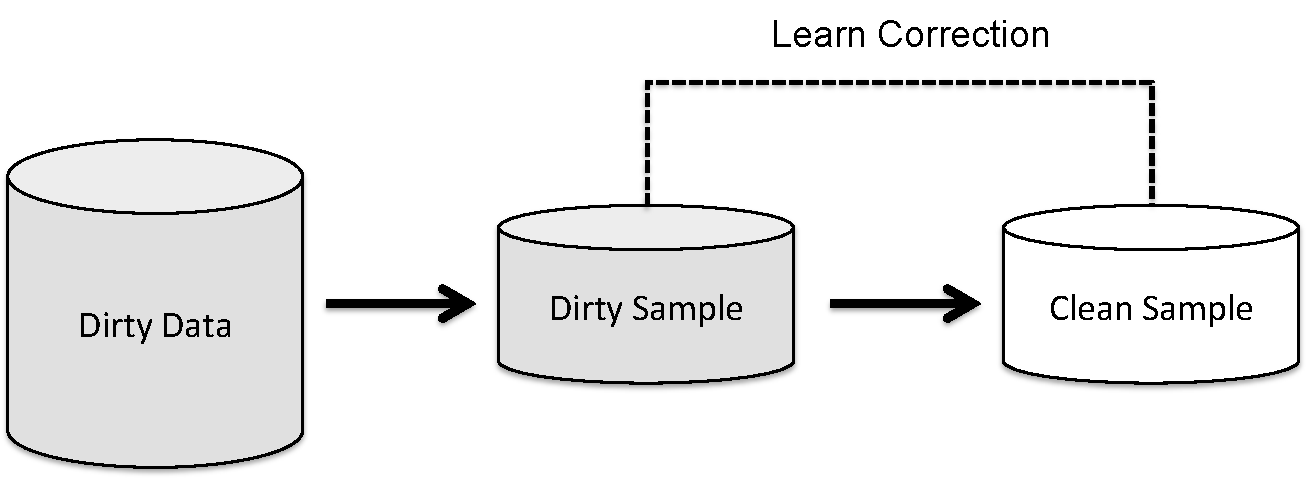
\includegraphics[scale=0.30]{figs/sys-arch2.pdf} \vspace{-.25em}
 \caption{A basic overview of SampleClean. SampleClean uses a random sample of dirty data to learn how a data cleaning algorithm affects queries on the sample. We can then derive a correction to compensate for the dirtiness. \reminder{You forgot to reference this figure in the text}}\vspace{-1.75em}
\end{figure}


{\noindent \bf Relationship to SAQP.}
Estimating the results of aggregate queries from samples has been
well studied in a field called Sample-based Approximate Query Processing
(SAQP) \cite{OlkenR86,AgarwalMPMMS13}.
Our approach differs from SAQP as we use a sample to correct a query rather than directly estimating the query result.
The SAQP approach to this problem, would be to
estimate the result directly from the maintained sample \cite{joshi2008materialized}.
We found that estimating
a correction and leveraging an existing deterministic result led
to lower variance results on real datasets (see Section \ref{exp}). 


